\chapter{An Incomplete Theory}
\label{sec:theo}

One of the great questions that humans have always tried to answer is
what are the fundamental building blocks of the universe and what are the rules that govern them?
Attempts at answering this question have ranged from
philosophical approach of \textit{`atomism'} by the ancient Greeks \cite{theo-atomism}
to the discovery of atomic structure by Ernest Rutherford \cite{theo-rutherford}.

The current best answer to this question is the \textit{`Standard Model of Particle Physics'},
a mathematical description of a finite set of fundamental particles and their interactions.
The Standard Model's ability to describe data is formidable
and as such it is the foundation of the field of particle physics. 
However, it is known that this is not a complete theory and there must be
a deeper underlying theory that lies beyond the Standard Model.

This chapter firstly aims to describe the Standard Model and its key predictions
with respect to the analyses within the context of this thesis.
Section~\ref{theo-sm} briefly describes the Standard Model and
Section~\ref{theo-qcd} outlines the QCD description of jet formation and dijet production in proton-proton collisions.
Then, Section~\ref{theo-bsm} will discuss physics Beyond the Standard Model (BSM);
specifically why it is thought that BSM physics is required
and what are some of the possible models that one can search for.

\newpage
\section{The Standard Model}
\label{theo-sm}

The Standard Model is a quantum field theory,
meaning that the theory describes a finite set of particles and their interactions in
terms of a set of fields.
The end product of the Standard Model is a prediction
of what will happen when any two particles in nature interact;
which in the context of a collider experiment means predicting what is the cross-section of any given interaction.

Section~\ref{theo-sm_particles} contains a description of the particles that make up the Standard Model 
and Section~\ref{theo-sm_forces} contains a description of the types of interactions between the particles, known as forces.

\subsection{Particles}
\label{theo-sm_particles}

There are 18 fundamental particles of the Standard Model,
where fundamental means that they are not composed of other constituent particles.
These particles are grouped into three families with similar properties;
known as quarks, leptons and bosons.
Details on the particles in the Standard Model is taken from~\cite{obj-bjets_PDG}, where a full description can be found.

\begin{itemize}[leftmargin=*]
\item\textbf{Quarks:}
  Quarks are fermions, meaning they are spin-$\frac{1}{2}$ particles,
  that interact with the strong force; a description of the strong force is in the next section.
  There are 6 different types of quarks, known as flavours, arranged in 3 generations.
  Table~\ref{tab:theo-sm_quarks} summarises the flavours of quark and their key properties.
  For each quark there is also an anti-quark, which has identical mass and spin, but opposite charge and quantum numbers.
  %\end{itemize}
  {\renewcommand{\arraystretch}{1.5}
  \begin{table}[!ht]
  \begin{center}
    \begin{tabular}{|c||c|c|c|c|}
      \hline
    Quark Flavour & Symbol & Charge            &  Spin           &  Mass [GeV]\\
    \hline
    Up            &   $u$  &  $+\frac{2}{3}$   &  $\frac{1}{2}$  &  0.02\\
    Down          &   $d$  &  $-\frac{1}{3}$   &  $\frac{1}{2}$  &  0.05\\
    \hline                                                   
    Charm         &   $c$  &  $+\frac{2}{3}$   &  $\frac{1}{2}$  &  1.3 \\
    Strange       &   $s$  &  $-\frac{1}{3}$   &  $\frac{1}{2}$  &  0.1 \\
    \hline                                                      
    Top           &   $t$  &  $+\frac{2}{3}$   &  $\frac{1}{2}$  &  173  \\
    Bottom        &   $b$  &  $-\frac{1}{3}$   &  $\frac{1}{2}$  &  4.2  \\
    \hline  
  \end{tabular}
    \caption{The key properties of the 6 flavours of quark in the Standard Model,
    organised into the three generations of quarks.}
  \label{tab:theo-sm_quarks}
  \end{center}
  \end{table}}

\item\textbf{Leptons:}
  Leptons are fermions that, unlike the quarks, do not interact with the strong force.
  There are 6 different types of leptons,
  arranged into  3 generations, each containing a charge $-1$ particle and a charge 0 neutrino.
  Table~\ref{tab:theo-sm_leptons} summarises the leptons and their key properties.
  The masses of the neutrinos are not well known, but they are known to be non-zero
  and the sum of the masses of the three flavours of neutrino is less than a few eV~\cite{theo-nu_mass}.
  For each lepton there is also an anti-lepton.
  
  {\renewcommand{\arraystretch}{1.5}
  \begin{table}[!ht]
  \begin{center}
    \begin{tabular}{|c||c|c|c|c|}
      \hline
    Lepton            & Symbol        & Charge  &  Spin           &  Mass [GeV]\\
    \hline
    Electron          &   $e$         &  -1    &  $\frac{1}{2}$   &  \num{5.1e-4}\\
    Electron Neutrino &   $\nu_e$     &  0     &  $\frac{1}{2}$   &  -\\
    \hline                                   
    Muon              &   $\mu$       &  -1    &  $\frac{1}{2}$   &  0.106 \\
    Muon Neutrino     &   $\nu_{\mu}$  &  0     &  $\frac{1}{2}$   &  -\\
    \hline                                      
    Tau               &   $\tau$       &  -1   &  $\frac{1}{2}$   &  1.8\\
    Tau Neutrino      &   $\nu_{\tau}$  &  0    &  $\frac{1}{2}$   &  -\\
    \hline  
  \end{tabular}
    \caption{The 6 types of lepton in the Standard Model and their key properties,
    organised into the three generations of leptons. Neutrino masses are not well known. }
  \label{tab:theo-sm_leptons}
  \end{center}
  \end{table}}
 
\item\textbf{Bosons:}
  The bosons are the set of spin-0 or spin-1 particles in the Standard Model,
  which act as the mediators of the forces that will be described below.
  Table~\ref{tab:theo-sm_bosons} summarises the bosons and their key properties.
  %The bosons are their own anti-particle, with the exception of the $W^{+}$ and $W^{-}$
  %which are each others anti-particle.

  {\renewcommand{\arraystretch}{1.5}
  \begin{table}[!ht]
  \begin{center}
    \begin{tabular}{|c||c|c|c|c|}
      \hline
    Boson            & Symbol        & Charge  &  Spin  &  Mass [GeV]\\
    \hline
    Photon           &   $\gamma$    &  0      &  1     &  0 \\
    W-boson          &   $W^{\pm}$    & $\pm$1  &  1     &  80 \\
    Z-boson          &   $Z_0$       &  0      &  1     &  91\\
    Gluon            &   $g$         &  0      &  1     &  0 \\
    Higgs Boson      &   $H$         &  0      &  0     &  125\\
    \hline  
  \end{tabular}
    \caption{The key properties of the bosons of the  Standard Model. }
  \label{tab:theo-sm_bosons}
  \end{center}
  \end{table}}
    
\end{itemize}

\subsection{Forces}
\label{theo-sm_forces}

The Standard Model combines three key theories in a
$SU(3)~\text{x}~SU(2)~\text{x}~U(1)$ gauge symmetry.
The first key theory is the electro-weak theory~\cite{theo-glashow};
this theory is based on mixing within the symmetry group $SU(2)~\text{x}~U(1)$
leading to three distinct interaction types grouped into two forces:
the electro-magnetic and weak forces.
The second is Quantum Chromodynamics (QCD)~\cite{theo-qcd} which describes the strong force.
Finally, the Brout-Englert-Higgs Mechanism~\cite{theo-be,theo-higgs} describes the origin of mass in the Standard Model.

\noindent
Each interaction is discussed in greater detail below:
\begin{itemize}[leftmargin=*]
\item\textbf{Electro-magnetic (EM):}

  The EM force is an interaction between charged particles and is mediated by the photon.
  The coupling is proportional to the product of the charges of the two particles
  multiplied by the EM coupling constant $\alpha_{EM}$, where $\alpha_{EM} \sim$ 1/137.\\ %\vspace{0.5em}

\item\textbf{Weak Force:}
  
  The weak force is composed of the two remaining interactions from electro-weak theory;
  the neutral current interaction and the charged current interaction.
  
  The neutral current interaction is mediated by the $Z_0$ boson, has a universal interaction to all fermions,
  and does not allow for flavour change within the interactions.

  The charged current interaction is mediated by the $W^+$ and $W^-$ boson, has a universal interaction with all fermions,
  and flavour changing interactions are allowed.
  Furthermore, due to the fact that the charged current interactions couples with weak eigenstates of fermions rather than
  their flavour eigenstates, the charged current interaction allows for interactions that change generation of the fermion's flavour.
  
  In the quark sector, the relative amplitudes of each flavour changing interactions is described by the CKM matrix;
  the structure of this matrix suppresses generational changing interactions,
  in particular those from the 3rd generation  are highly suppressed.
  This feature will prove important for identifying the presence of $b$-quarks at the ATLAS detector.
  Both interactions of the weak force are much weaker than the EM force due to the large masses of the mediating particles
  (\text{Weak}/\text{EM} \sim 10^{-4}$).\\ %\vspace{0.5em}
  
\item\textbf{Strong Force:}

  Quantum Chromodynamics (QCD) is a theory described by a SU(3) gauge symmetry that describes the interactions between quarks and gluons.
  The symmetry leads to 3 colour charges: known as red, green and blue.
  If an object contains all three colour charges then it is a colour neutral object.
  The strong force is mediated by the gluon and interacts with particles that have colour charge; which are quarks and gluons.
  The fact that the gluon has colour charge means that the gluon is self interacting.
  QCD is important in terms of understanding jet formation and the production of the
  largest background in a dijet search, so further details can be found in section in Section~\ref{theo-qcd}.\\

\item\textbf{Higgs Mechanism:}
  The Higgs Mechanism \footnote{Also known as the Higgs-Englert-Brout mechanism}
  introduces an extra scalar field to the Standard Model
  and a Higgs potential given by the so-called `Mexican-hat potential'.
  This allows for spontaneous symmetry breaking which gives mass to the bosons of the Standard Model.
  In addition, a Yukawa coupling term between the scalar field and the fermions gives rise to the mass of the fermions
  \footnote{With the exception of the neutrinos, whose mass is not described by the Standard Model}.
  A final prediction of the Higgs mechanism was the existence of a spin-0 boson, known as the Higgs boson.
  The first observation of the Higgs Boson like object by the ATLAS~\cite{theo-higgs_atlas} and CMS~\cite{theo-higgs_cms} experiments
  in 2012 appears to confirm the Higgs mechanism, which would be a great triumph of the Standard Model.
\end{itemize}

\section{QCD: Jet Formation and Dijet Production}
\label{theo-qcd}

As described above Quantum Chromodynamics (QCD) is a theory that describes the strong interaction between
quarks and gluons.
QCD therefore describes two elements that are critical to the analysis being presented in this thesis;
specifically the formation of jets and the production of dijet events through QCD in proton-proton collisions,
which will be the dominant background in the analysis.

This section will firstly describe renormalisation of QCD, which is important for understanding how QCD works,
and will then describe the process of jet formation and dijet production in hadron collisions.
Quarks and gluons can often fill similar roles in jet formation and dijet production, hence I will refer to them collectively as `partons' in this section.

\subsection{Renormalisation and the Running of $\alpha_S$}
\label{sec:theo-qcd_dijet_running}

For any calculation in QCD, or indeed any quantum field theory, one must consider the higher order loop diagrams;
for example for a simple gluon propagator there are additional first-order loops as shown in Figure~\ref{fig:theo-qcd_gluon}.
These additional loops lead to divergences in calculations of scattering events in QCD.

\begin{figure}[!hbt]
  \begin{center}
    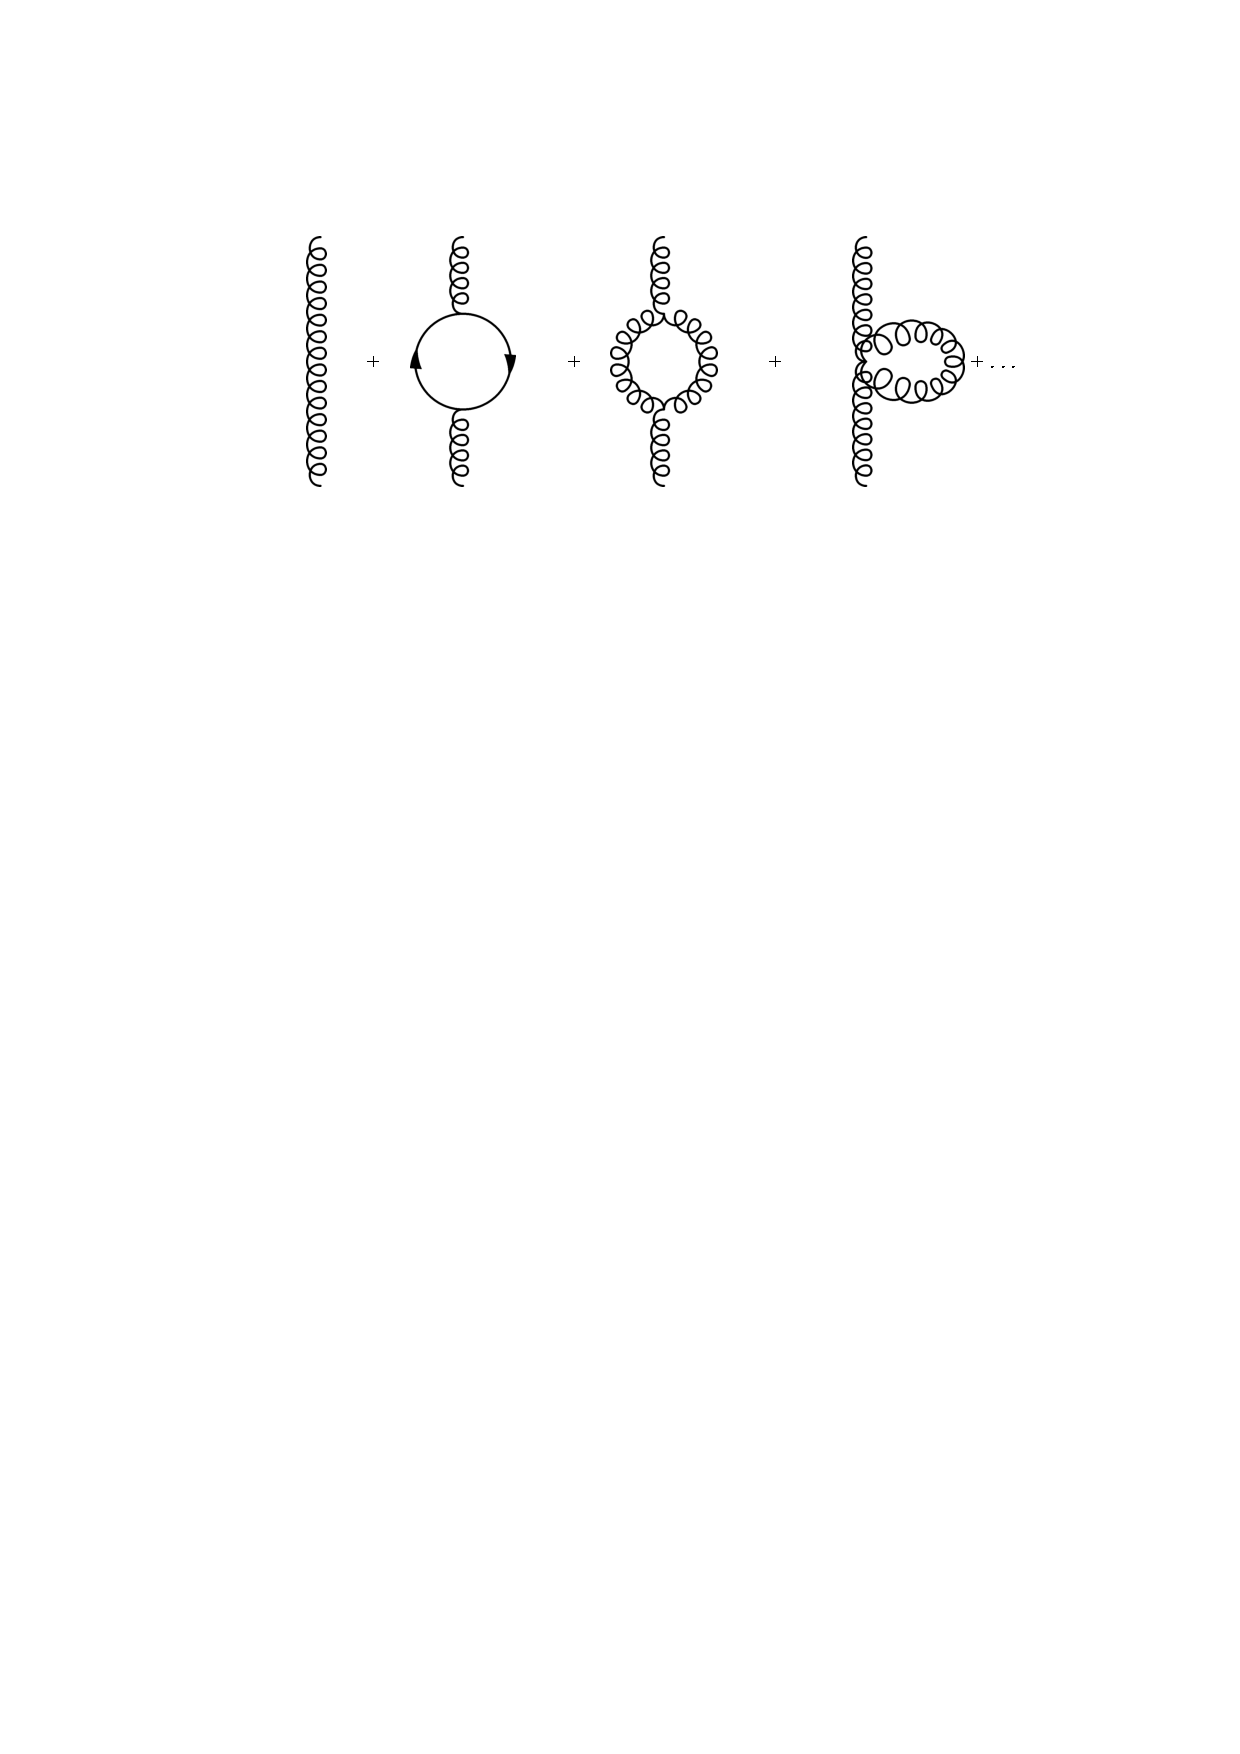
\includegraphics[width=0.7\linewidth, angle=0]{figs/Theory/qcd_gluon_loop.pdf}
  \end{center}
  \caption[A schematic showing the gluon propagator with the additional first order loops.]
  {A schematic showing the gluon propagator with the additional first order loops~\cite{det-thesis_kate}.}
  \label{fig:theo-qcd_gluon}
\end{figure}

To avoid these divergences, there is a well accepted mathematical tool known as renormalisation,
where one effectively re-scales the fields in the Lagrangian.
This is done such that the divergences are removed
and one can perform calculations of QCD in a perturbative expansion.
This leads to a dependence of the strong coupling, $\alpha_S$, on the renormalisation scaled used, $\mu_R$,
an effect known as the running of $\alpha_S$.
To get an effective strength of the strong interaction in any given process,
$\mu_R$ is set close to the scale of the momentum transfer $Q$ of the process.
%$\alpha_S($\mu_R \sim Q^{2}$).
The running of $\alpha_S$ can be measured through experimental observation;
Figure~\ref{fig:theo-qcd_running} shows the measured values of
the strong coupling constant, $\alpha_S$ as a function of the energy scale, $Q$, in a range of experiments.

\begin{figure}[!hbt]
  \begin{center}
    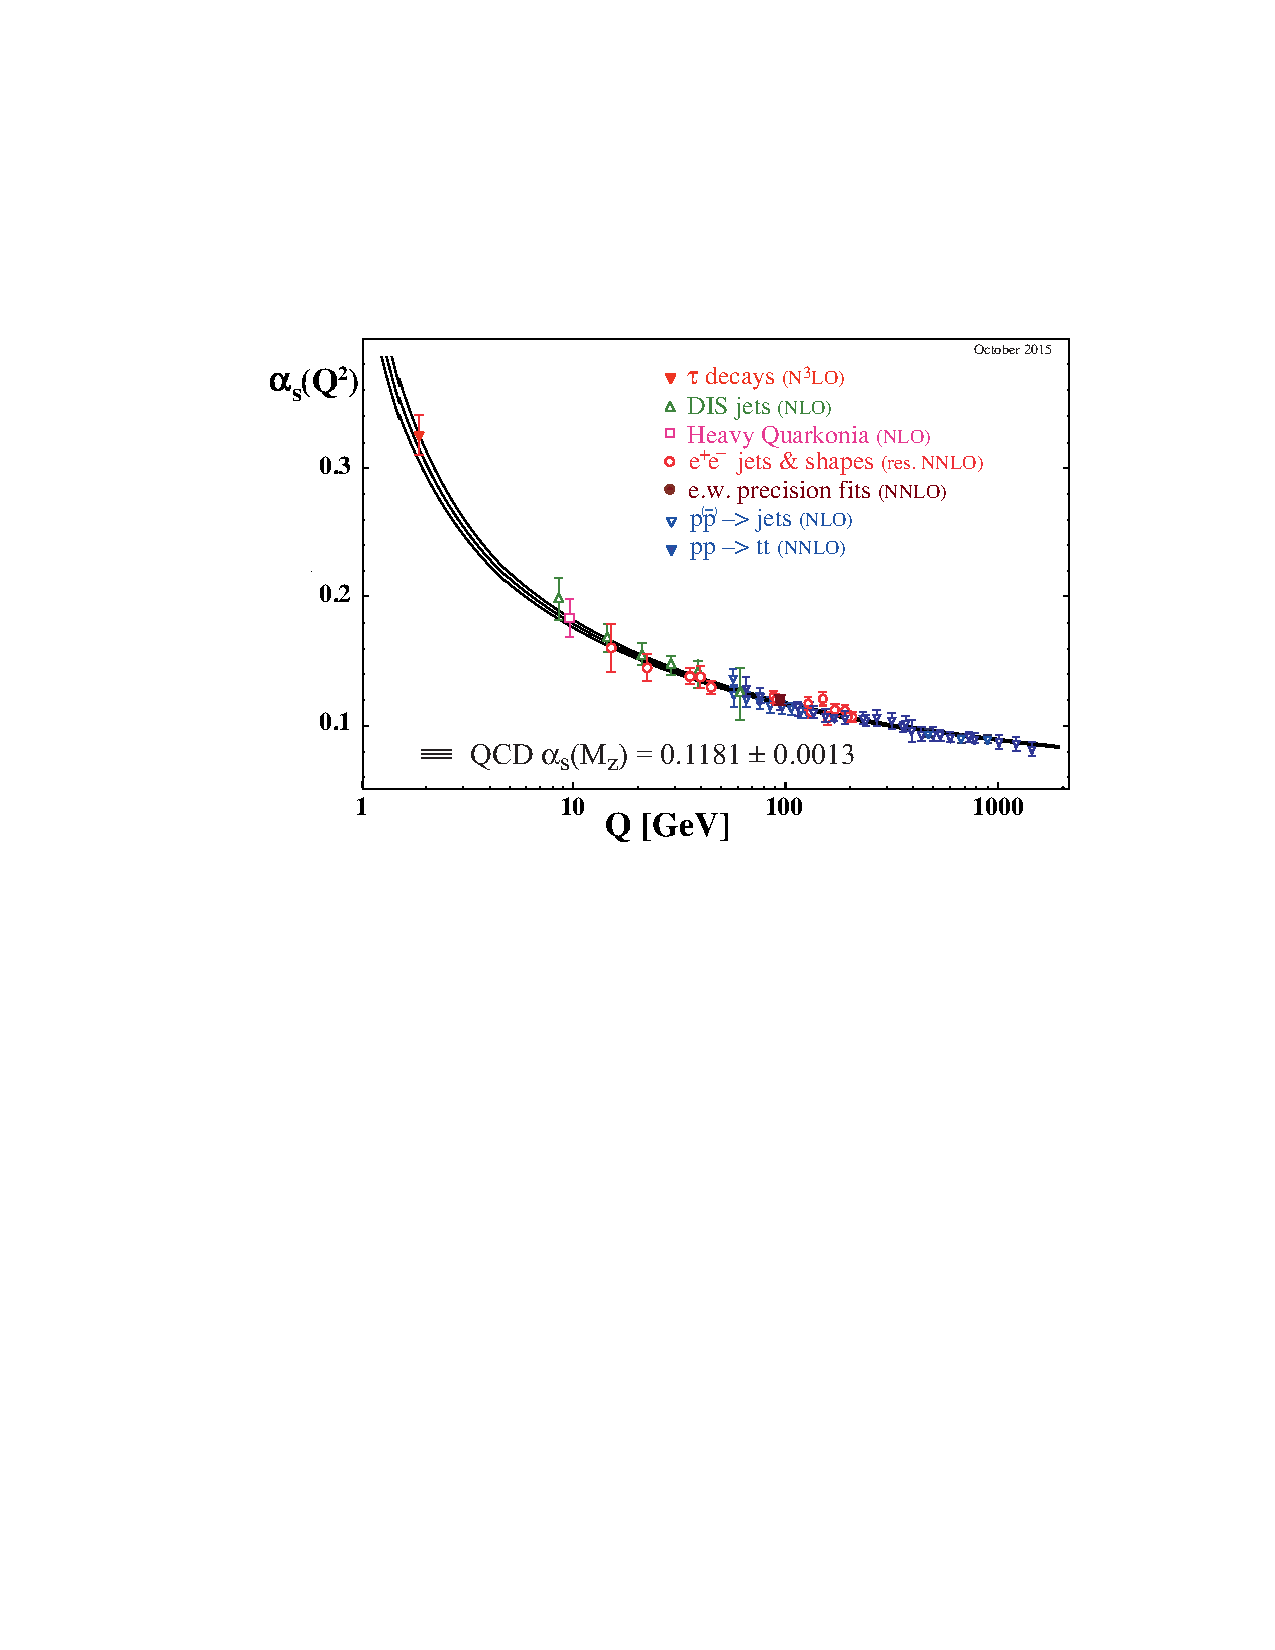
\includegraphics[width=0.7\linewidth, angle=0]{figs/Theory/qcd_running.pdf}
  \end{center}
  \caption[Summary of measurements of $\alpha_S$ as a function of the energy scale $Q$.
    The respective degree of QCD perturbation theory used in the extraction of $\alpha_S$ is indicated in brackets
    (NLO: next-to-leading order; NNLO: next-to-next-to leading order; res. NNLO: NNLO matched with resummed next-to-leading logs; N3LO: next-to-NNLO).]
          {Summary of measurements of $\alpha_S$ as a function of the energy scale $Q$.
            The respective degree of QCD perturbation theory used in the extraction of $\alpha_S$ is indicated in brackets
            (NLO: next-to-leading order; NNLO: next-to-next-to leading order; res. NNLO: NNLO matched with resummed next-to-leading logs; N3LO: next-to-NNLO)~\cite{theo-qcd}.}
  \label{fig:theo-qcd_running}
\end{figure}

There are three features of Figure~\ref{fig:theo-qcd_running} that can be noted.
Firstly that the size of the coupling constant, $\alpha_S$, is large compared to the
$\alpha_{EM} \sim 1/137$;
this means that the strong force is stronger than the $EM$ force by at least an order of magnitude.
Secondly, at high-energies/low-distance scales the strong force becomes weak, such the quarks and gluons barely interact, this phenomenon is known as
\textit{`assymptotic freedom'}.
At these energy scales, pertubative expansions of QCD are possible.
Finally, at low-energies/large-distance scales the strong force is exceptionally strong.
As a result, if two interacting quarks become seperated by a large distance then it becomes energetically favourable to
pair-produce a $q\bar{q}$ pairs from the vacuum until a colour neutral object can be formed.
Therefore quarks will never be observed in isolation but instead quarks form colour neutral hadrons, this feature of QCD is known as \textit{`confinement'}.

\subsection{Jet Formation}
\label{sec:theo-qcd_jets}

It is common in hadronic colliders that a high-momentum quark or gluon will be produced in the final-state,
an example of this is the dijet production described in Section~\ref{sec:theo-qcd_dijet}.
However, as described in Section~\ref{sec:theo-qcd_dijet_running},
the large values of $\alpha_S$ at large distance-scales require quark confinement, meaning that an isolated quark or gluon will not be observed.
Instead a jet of energetic hadrons, known as hadronic jet, will be formed.
Hadronic formation is described by two distinct processes; parton-shower and hadronisation.

\begin{itemize}[leftmargin=*]
\item\textbf{Parton Shower:}

  The high-energy final-state quark or gluon has a finite probability of splitting into a quark-gluon or quark-quark pair.
  The resulting quarks and gluons will also undergo splitting to form more partons and this process repeats to form a shower.
  Due to relativistic effects, each splitting will generally be at a small angle in the lab-frame
  and as such the partons will highly collimated to the direction of the intial parton.
  The parton shower process is at high energy such that the value of $\alpha_S$ is small
  and thus pertubative expansions of QCD can be used to perform calculations.
  However, at each step of the splitting the energy of the partons decreases such that $\alpha_S$ increases.
  
\item\textbf{Hadronisation:}
  
  When $\alpha_S$ becomes large, confinement becomes the dominant effect in a QCD interaction.
  Therefore, the quarks resulting from the parton shower will form baryons which are colour netural objects.
  The colour neutral baryons will not interact though QCD and hence will be relatively stable.
  \footnote{Weak interactions can still occur; such that not all baryons formed are totally stable}
  The hadronisation process occurs at large values of $\alpha_S$ so cannot be calculated using pertubative expansions;
  to simulate QCD models such as the string model~\cite{theo-qcd_jet_string} and the
  cluster model~\cite{theo-qcd_jet_cluster} are used to approximate the hadronisation step.

\end{itemize}
  
The end result of the hadronisation process is a set of highly collimated stable baryons,
known as a hadronic jet, which can be observed in an experiment.
Note that our understanding of how one goes from an initial parton to a hadronic is model dependant,
for example your choice of hadronisation model;
hence in experiment we remove this dependance by defining a jet in terms of observables.
The jet observables and the experimental definition of a jet used is discussed in~\ref{sec:obj-jets}.

%\subsection{Parton shower}
%\subsection{Hadronisation}

\subsection{Dijet Production in $pp$ Collisions}

Dijet production is one of the most common process that occurs in any hadron collider.
The first step of dijet production in $pp$ colliders is the two protons interacting through QCD to give two quarks or gluons in the final state;
the relative frequency of this interaction is described by the hadronic cross-section, $\sigma_{had}$.
The free partons will then form hadronic jets through the processes described in Section~\ref{sec:theo-qcd_jets}.
As an example, Figure~\ref{fig:theo-qcd_dijet_feynman} shows the Feynman diagram of
dijet production in a proton-proton collision through one of the modes, the qg$\to$qg channel.

\begin{figure}[!hbt]
  \begin{center}
    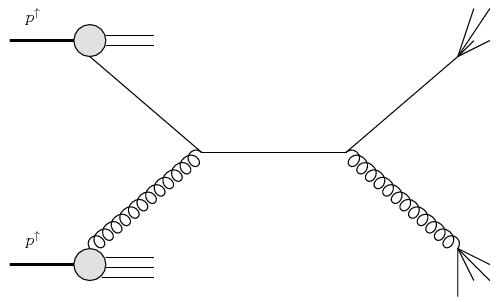
\includegraphics[width=0.7\linewidth, angle=0]{figs/Theory/qcd_dijet_feynman.png}
  \end{center}
%  \caption[Three feynman diagrams illustrating the parton level scatter process in dijet production at the LHC.]
%          {Three feynman diagrams illustrating the parton level scatter process in dijet production at the LHC~\cite{theo-qcd_dijet_feynman}.}
  \caption[A Feynman diagram showing dijet production in a proton-proton collision through the qg$\to$qg channel.]
          {A Feynman diagram showing dijet production in a proton-proton collision through the qg$\to$qg channel~\cite{theo-qcd_dijet_feynman}.}
  \label{fig:theo-qcd_dijet_feynman}
\end{figure}

\subsubsection{Factorisation}

To calculate the hadronic cross-section, $\sigma_{had}$, in a proton-proton collision,
two elements are separated out in a process called factorisation.

The first element is the parton-level cross-section, $\hat{\sigma}$, which is the cross-section of
two partons from the proton ($p_a$ and $p_b$) scattering to give two final state partons ($p_i$ and $p_j$).
This is effectively the central part of the Feynman diagram in Figure~\ref{fig:theo-qcd_dijet_feynman}.

The second element is the Parton Density Functions (PDFs), $f_a(x_a)$, which described the probability of
a proton yielding a parton, $p_a$, with momentum fraction, $x_a$.
Momentum fraction is defined as the fraction of the protons total momentum that the parton is carrying, $x = p_{\text{parton}}/p_{\text{proton}}$.

The elements are combined to calculate the total $\sigma_{had}$;
\begin{equation}
%  \sigma(p_1p_2\to q/g_i q/g_j) = \int dx_1 dx_2 f_1(x_1,\mu^2_F)f_2(x_2\mu^2_F) \sigma(q/g_1,q/g_2, \alpha_s(\mu^2_R),Q^2/\mu^2_F,Q^2/\mu^2_R)
  \sigma_{had} = \sum_{a,b,i,j} \int dx_a dx_b f_a(x_a,Q^2)f_b(x_b,Q^2) \hat{\sigma}(p_a, p_b\to p_i p_j)
\end{equation}
where there is an integral over all possible values of momentum fractions $x_a$ and $x_b$,
a sum over all possible partons from the two protons labelled $a$ and $b$,
and a sum over all possible final-state partons labelled by $i$ and $j$.
$Q^2$ is the energy scale of the collision.

With the two elements separated we can discuss each separately.

\subsubsection{Parton-level Cross-Section}
\label{sec:theo-qcd_dijet_xs}

To describe the parton-level cross-section we must first define a few variables.
The first is the invariant mass of the outgoing partons, $m_{ij}$, which is given in terms of the four-momentum of the two partons by;
\begin{equation}
  m_{ij}^2 = (p^\mu_i + p^\mu_j)^2  
\end{equation}
\noindent
Then there are two related angular variables, $y^*$ and $\theta^*$,
defined in terms of $y_i$, the rapidity of the outgoing parton $p_i$;
\begin{equation}
  y^* = (\frac{y_i - y_j}{2}),
\end{equation}
\begin{equation}
  cos(\theta^*) = \tanh(y^*)
\end{equation}
\noindent
Finally the Mandelstam variables, generally used to describe a 2$\to$2 particle scatter event, are defined as 
\begin{equation}
  \hat{s} = m_{ij}^2, \hspace{3mm}  \hat{t} = -\hat{s}\hspace{1mm}(1 - \cos{\theta^*}), \hspace{3mm} \hat{u} = - \hat{s}\hspace{1mm}(1+\cos{\theta^*})
\end{equation}

\noindent
The parton-level cross-section of incoming partons $a$ and $b$ scattering to give
outgoing partons $i$ and $j$ is given in terms of the variables $\theta^*$ and $m_{ij}$~\cite{theo-dijet_harris};
\begin{equation}
  \frac{d\hat{\sigma}(p_a, p_b \to p_i p_j)}{dm_{ij}\hspace{1mm}d\cos{\theta^*}} = \frac{ \pi \alpha_s}{m_{ij}}\hspace{1mm} \text{S}(ab \to ij) \hspace{1mm} \frac{1}{1+\delta_{ij}}
  \label{eq:theo-qcd_dijet_xs}
\end{equation}
Where $\text{S}(ab \to ij)$ gives the process dependant kinematics of a $ab \to ij$  parton scatter.
$\text{S}(ab \to ij)$ for each process is described in Table~\ref{tab:theo-qcd_dijet_s}.

%  {\renewcommand{\arraystretch}{1.5}
%  \begin{table}[!ht]
%  \begin{center}
%    \begin{tabular}{|c|c|}
%      \hline
%      Subprocess         & $\text{S}(ab \to ij)$ \\
%    q1q2 - q1q2          &    4 s + u / 9t       \\
%    q1barq2 - q1barq2    &    4 s + u / 9t       \\
%    q1q1 - q1q1          &    4 s + u / 9t +  4 s + t / 9u
%    q1barq1 - q2barq2
%    
%    \hline  
%  \end{tabular}
%    \caption{The key properties of the 6 flavours of quark in the Standard Model,
%    organised into the three generations of quarks.}
%  \label{tab:theo-sm_quarks}
%  \end{center}
%  \end{table}}
%

\begin{table}[!hbt]
  \begin{center}
    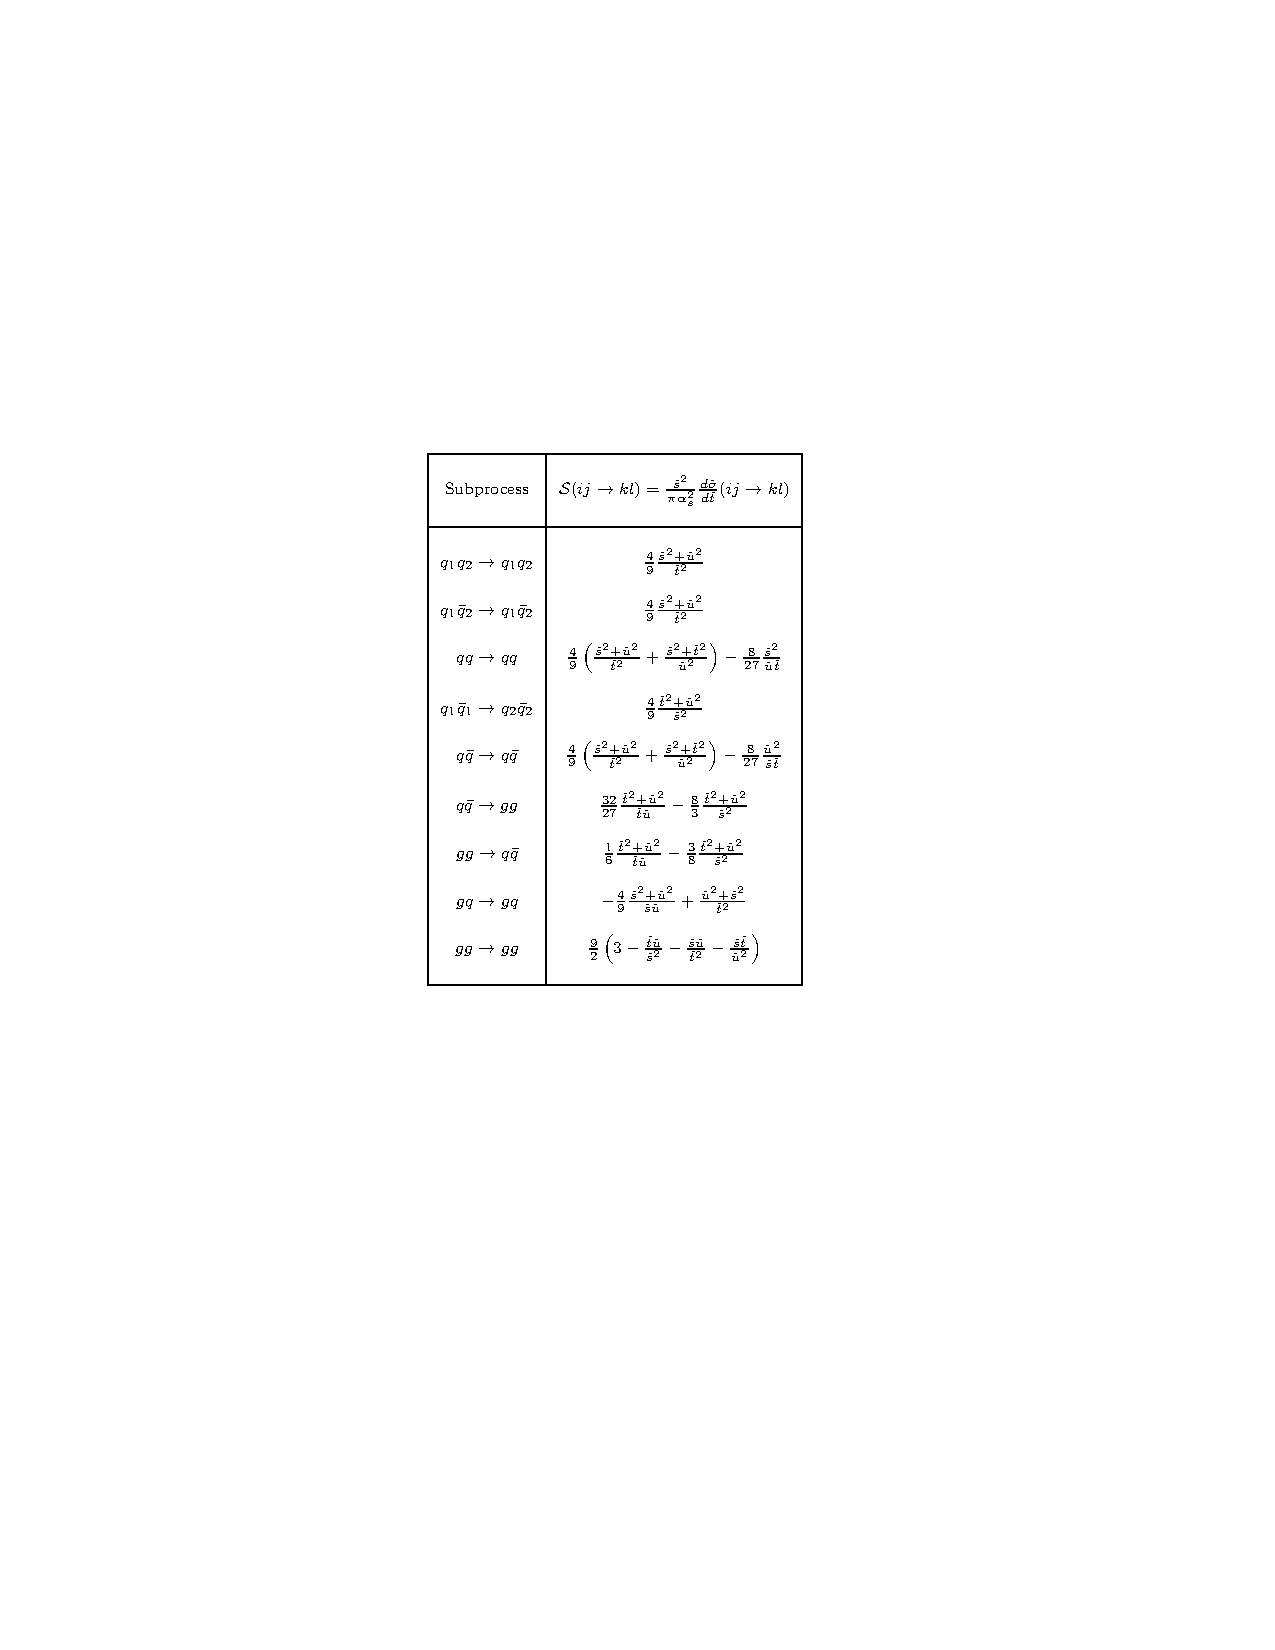
\includegraphics[width=0.7\linewidth, angle=0]{figs/Theory/qcd_dijet_stable.pdf}
  \end{center}
  \caption[A table showing the process dependant part of the parton cross-section, $\text{S}(ab \to ij)$, for each of the processes in dijet production.]
  {A table showing the process dependant part of the parton cross-section, $\text{S}(ab \to ij)$, for each of the processes in dijet production. Taken from Table 1 of~\cite{theo-dijet_harris}.}
  \label{tab:theo-qcd_dijet_s}
\end{table}

\newpage
\subsubsection{Parton Density Functions}
\label{sec:theo-qcd_pdf}

Parton Density Functions (PDFs) describe effectively what is the probability of finding a parton $p_a$ in a proton $P_a$
for a given momentum fraction $x_a$ and energy scale, $Q$.
They have been studied extensively
by combining experimental scattering measurements,
particularly from deep inelastic scattering using $ep$ colliders such as HERA~\cite{theo-qcd_hera}.

Figure~\ref{fig:theo-qcd_pdf} shows the $x\hspace{0.3mm}F(x,Q^2)$ for a $Q^2$ of 10 and $10^4$ $\text{GeV}^2$
from the MMHT2014 PDF set~\cite{theo-qcd_pdf}.
The various colours lines represent the PDF for each of the different partons.

\begin{table}[!hbt]
  \begin{center}
    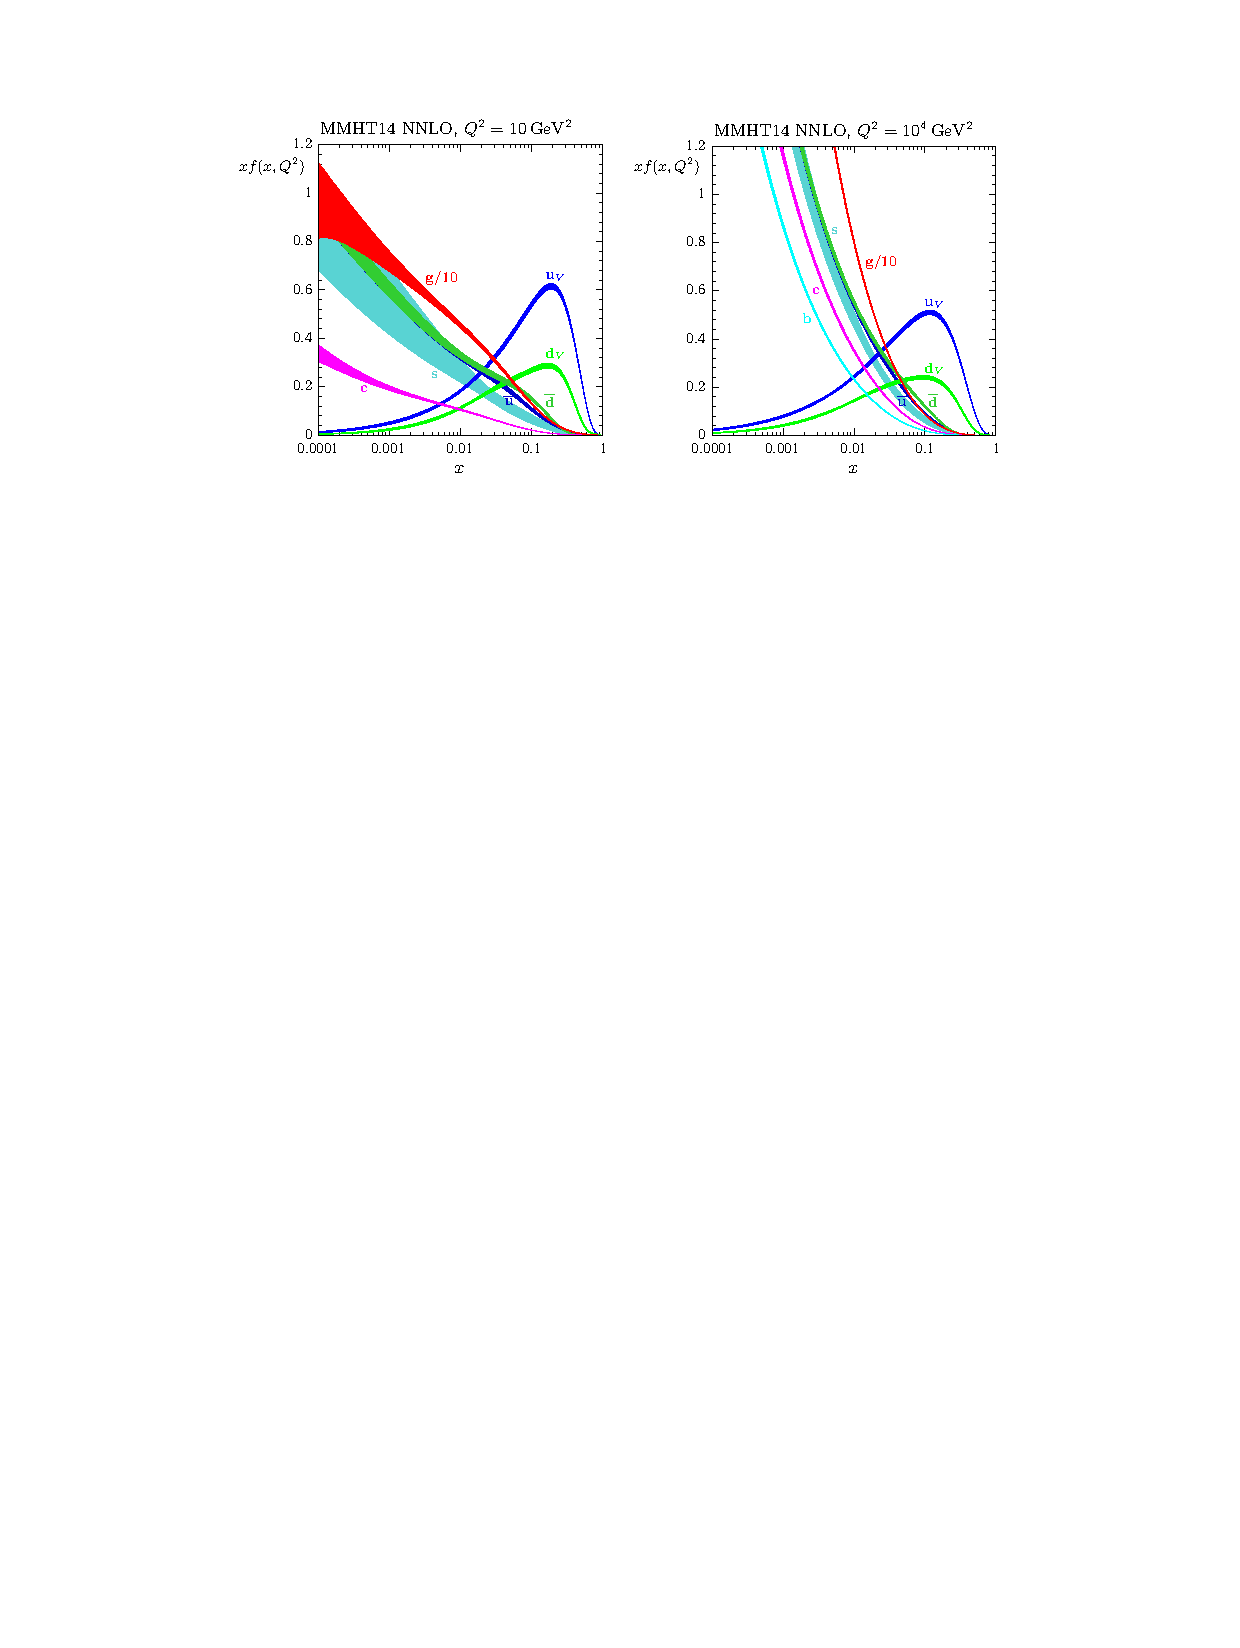
\includegraphics[width=1\linewidth, angle=0]{figs/Theory/qcd_pdf.pdf}
  \end{center}
  \caption[MMHT2014 NNLO PDFs at $Q^2$ = 10 $\text{GeV}^2$ and $Q^2$ = $10^4$ $\text{GeV}^2$, with associated 68\% confidence-level uncertainty bands.]
  {MMHT2014 NNLO PDFs at $Q^2$ = 10 $\text{GeV}^2$ and $Q^2$ = $10^4$ $\text{GeV}^2$, with associated 68\% confidence-level uncertainty bands~\cite{theo-qcd_pdf}.}
  \label{fig:theo-qcd_pdf}
\end{table}


One can note that as $x$ increases the values of the PDF for the quarks and gluons will fall smoothly.
This is particularly notable for the gluon which is the dominant contribution at low values of $x$.
The exception to this general behaviour is the valence quarks,
$u_v$ and $d_v$,
which are the quarks that are typically seen as the constituents of a proton and have a peak value around $x \sim \frac{1}{3}$.

\subsubsection{Features of the Hadronic Cross-section}

There are three important features that one can qualitatively describe about the dijet hadronic cross-section
from the two factorised elements shown in Section~\ref{sec:theo-qcd_dijet_xs}~and~\ref{sec:theo-qcd_pdf}.
These important features will have significance when forming the dijet search analysis strategy in
Chapters~\ref{bkg}\textit{Background estimation chapter} and~\ref{evt}\textit{Event selection chapter}.

\begin{itemize}[leftmargin=*]
\item\textbf{Large cross-section :}\\
  The strong coupling constant $\alpha_s$ is much larger than the other forces,
  meaning that the dijet cross-section is large.
  As a result dijet production through QCD is one of the most common events at hadron colliders
  and will be the strongly dominant background in any dijet search.\vspace{0.5em}
\item\textbf{Behaviour with respect to $m_{ij}$ :}\\
  It can be seen that hadronic cross-section will
  lead to a smooth and monotonically decreasing spectrum
  with respect to $m_{ij}$ as a result of three factors.
  Firstly the cross section has a $1/m_{ij}$ term.
  Secondly, as shown in Section~\ref{sec:theo-qcd_dijet_running},
  $\alpha_S$ will smoothly decrease with increasing $Q$, which in this case is linked to $m_{ij}$.
  Finally, as $m_{ij}$ increases then the momentum fraction of the proton, $x$, required to create
  the dijet event will also increase.
  As shown in Figure~\ref{fig:theo-qcd_pdf}, the parton density function of the quarks and the gluon
  is smoothly falling as $x$ increases, which will lead to falling behaviour in the hadronic cross-section.
  \vspace{0.5em}
\item\textbf{Behaviour with respect to $y^*$ :}\\
  In all but one of the $\text{S}(ab \to ij)$ terms shown in Table~\ref{tab:theo-qcd_dijet_s},
  we see that, due to the $t$-channel diagram, there is a $1/\hat{t}$ term that will become large when $\cos{\theta^*} \to 1$.
  Hence, we find that there is a larger dijet cross-section at large values of $\cos{\theta^*}$ and $y^*$.
  \vspace{0.5em}
\end{itemize}

Finally it should be noted that the above description of the dijet cross-section is
not a full description of the QCD interactions at hadron-hadron collisions.
Here I have only considered the tree-level diagrams;
one needs to consider higher orders of perturbative QCD to give a fuller description of dijet production.
Related to that issue is the problems of initial state and final state radiation, known as ISR and FSR respectively.
ISR is when an additional parton is radiated of the incoming parton where FSR is when an additional parton is radiated of the outgoing parton,
which can lead to additional jets in an event, creating a multi-jet event.

One should also consider the Underlying Event (UE) which effectively comprises of the remnants of the proton not used in the hard-scatter.
The UE will mostly be hadronic activity and as a result can lead to additional jets in the event, again giving us a multi-jet event.



\subsection{A Special Case: $t\bar{t}$}



\section{Beyond the Standard Model}
\label{theo-bsm}

\subsection{Why do we need BSM}
\subsection{Benchmark models}
\subsubsection{$Z'$ Boson}
\subsubsection{Excited $b^*$ quark}
